% Native 3.8 cm panels; four stations by reference and three models.
\begin{subfigure}{0.24\textwidth}\centering
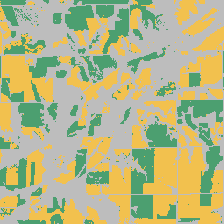
\includegraphics{results/fig_within_site_errors_A_reference.pdf}
\caption{A站参考标签}
\end{subfigure}\hfill
\begin{subfigure}{0.24\textwidth}\centering
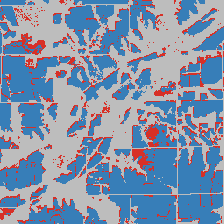
\includegraphics{results/fig_within_site_errors_A_convgru.pdf}
\caption{A站ConvGRU对错图}
\end{subfigure}\hfill
\begin{subfigure}{0.24\textwidth}\centering
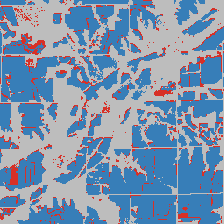
\includegraphics{results/fig_within_site_errors_A_unet3d.pdf}
\caption{A站3D U-Net对错图}
\end{subfigure}\hfill
\begin{subfigure}{0.24\textwidth}\centering
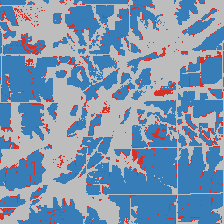
\includegraphics{results/fig_within_site_errors_A_utae.pdf}
\caption{A站U-TAE对错图}
\end{subfigure}\par\nointerlineskip\vspace{3pt}
\begin{subfigure}{0.24\textwidth}\centering
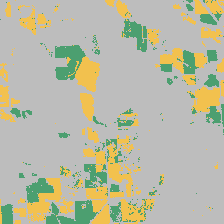
\includegraphics{results/fig_within_site_errors_B_reference.pdf}
\caption{B站参考标签}
\end{subfigure}\hfill
\begin{subfigure}{0.24\textwidth}\centering
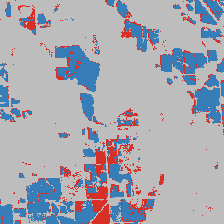
\includegraphics{results/fig_within_site_errors_B_convgru.pdf}
\caption{B站ConvGRU对错图}
\end{subfigure}\hfill
\begin{subfigure}{0.24\textwidth}\centering
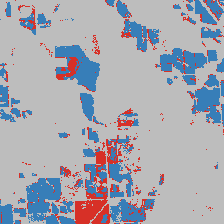
\includegraphics{results/fig_within_site_errors_B_unet3d.pdf}
\caption{B站3D U-Net对错图}
\end{subfigure}\hfill
\begin{subfigure}{0.24\textwidth}\centering
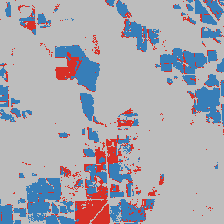
\includegraphics{results/fig_within_site_errors_B_utae.pdf}
\caption{B站U-TAE对错图}
\end{subfigure}\par\nointerlineskip\vspace{3pt}
\begin{subfigure}{0.24\textwidth}\centering
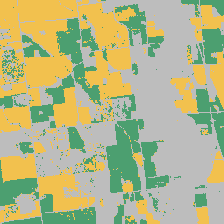
\includegraphics{results/fig_within_site_errors_C_reference.pdf}
\caption{C站参考标签}
\end{subfigure}\hfill
\begin{subfigure}{0.24\textwidth}\centering
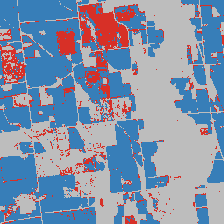
\includegraphics{results/fig_within_site_errors_C_convgru.pdf}
\caption{C站ConvGRU对错图}
\end{subfigure}\hfill
\begin{subfigure}{0.24\textwidth}\centering
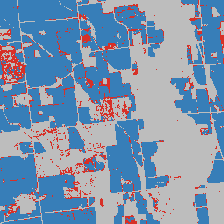
\includegraphics{results/fig_within_site_errors_C_unet3d.pdf}
\caption{C站3D U-Net对错图}
\end{subfigure}\hfill
\begin{subfigure}{0.24\textwidth}\centering
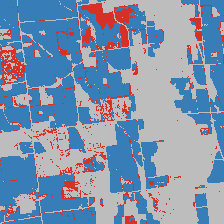
\includegraphics{results/fig_within_site_errors_C_utae.pdf}
\caption{C站U-TAE对错图}
\end{subfigure}\par\nointerlineskip\vspace{3pt}
\begin{subfigure}{0.24\textwidth}\centering
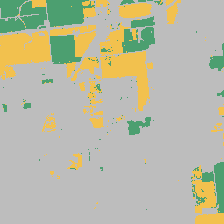
\includegraphics{results/fig_within_site_errors_D_reference.pdf}
\caption{D站参考标签}
\end{subfigure}\hfill
\begin{subfigure}{0.24\textwidth}\centering
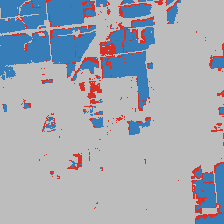
\includegraphics{results/fig_within_site_errors_D_convgru.pdf}
\caption{D站ConvGRU对错图}
\end{subfigure}\hfill
\begin{subfigure}{0.24\textwidth}\centering
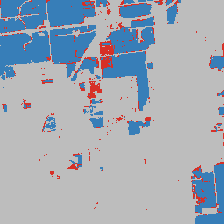
\includegraphics{results/fig_within_site_errors_D_unet3d.pdf}
\caption{D站3D U-Net对错图}
\end{subfigure}\hfill
\begin{subfigure}{0.24\textwidth}\centering
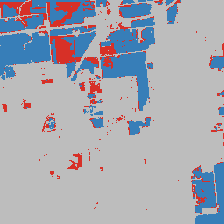
\includegraphics{results/fig_within_site_errors_D_utae.pdf}
\caption{D站U-TAE对错图}
\end{subfigure}\par\nointerlineskip\vspace{3pt}
\definecolor{sec31Correct}{HTML}{377EB8}
\definecolor{sec31Error}{HTML}{D73027}
{\songti\zihao{-5}参考标签：\legbox{cCorn}\,玉米\quad\legbox{cSoy}\,大豆\quad\legbox{cOther}\,其它地类\par}
\nointerlineskip\vspace{3pt}
{\songti\zihao{-5}对错图：\legbox{sec31Correct}\,正确作物像元\quad\legbox{sec31Error}\,错分作物像元\quad\legbox{cOther}\,参考其它地类\quad
\begin{tikzpicture}[x=0.494791667cm,y=1cm,baseline=-0.7ex]
\draw[line width=0.6pt] (0,0)--(2,0);
\foreach \x in {0,1,2} {\draw[line width=0.6pt] (\x,0)--(\x,0.07);}
\node[anchor=north,font=\songti\zihao{-5},inner sep=1pt] at (0,0) {0};
\node[anchor=north,font=\songti\zihao{-5},inner sep=1pt] at (1,0) {1};
\node[anchor=north west,font=\songti\zihao{-5},inner sep=1pt] at (2,0) {2 km};
\end{tikzpicture}\par}
